%%%%%%%%%%%%%%%%%%%%%%%%%%%%%%%%%%%%%%%%%
% University Assignment Title Page 
% LaTeX Template
% Version 1.0 (27/12/12)
%
% Original author:
% WikiBooks (http://en.wikibooks.org/wiki/LaTeX/Title_Creation)
%
% License:
% CC BY-NC-SA 3.0 (http://creativecommons.org/licenses/by-nc-sa/3.0/)
%
%%%%%%%%%%%%%%%%%%%%%%%%%%%%%%%%%%%%%%%%%

%----------------------------------------------------------------------------------------
%	PACKAGES AND OTHER DOCUMENT CONFIGURATIONS
%----------------------------------------------------------------------------------------

\documentclass[12pt]{article}
\usepackage[english]{babel}
\usepackage[utf8]{inputenc}
\usepackage{amsmath}
\usepackage{amsfonts}
\usepackage{graphicx}
\usepackage{color}
\usepackage{ifpdf}
\usepackage[plainpages=false,colorlinks=true,pdfpagelabels,pdfborderstyle={/S/U/W 1}]{hyperref}

% 
% Meta information of the project paper
% 

% Title of the project
\newcommand{\projecttitle}{Title of the Project}

% Name of the authors
\newcommand{\authorsTitle}{
	Aaron \textsc{}\\
	Jan \textsc{Keesen}
}
\newcommand{\authors}{Aaron and Jan Keesen}

% Name of the university
\newcommand{\university}{Ludwig-Maximilians-Universität München}

% Name of the course
\newcommand{\course}{Computational finance with a view to Octave/MATLAB implementation}

% Name of the lecturer
\newcommand{\lecturer}{Dr.~Lorenzo~\textsc{Torricelli}}

% Define pdf meta
\ifpdf
	\definecolor{bwblue}{rgb}{0.317,0.161,1}
    \hypersetup{
      pdftitle={\projecttitle},
      pdfsubject={Project assignment},
      pdfauthor={\authors},
      urlcolor=bwblue,
      citecolor=black,
    }
\else   
\fi

\newcommand{\C}{C_{BS}}
\newcommand{\p}{\partial}

\begin{document}

\begin{titlepage}

\newcommand{\HRule}{\rule{\linewidth}{0.5mm}} % Defines a new command for the horizontal lines, change thickness here

\center
 
%----------------------------------------------------------------------------------------
%	HEADING SECTIONS
%----------------------------------------------------------------------------------------

\textsc{\LARGE \university}\\[1.5cm] % Name of the university
\textsc{\Large \course}\\[0.5cm] % Major heading
\textsc{\large Project assignment}\\[0.5cm] % Minor heading

%----------------------------------------------------------------------------------------
%	TITLE SECTION
%----------------------------------------------------------------------------------------

\HRule \\[0.5cm]
{ \huge \bfseries \projecttitle}\\ % Title of the document
\HRule \\[0.5cm]
 
%----------------------------------------------------------------------------------------
%	AUTHOR SECTION
%----------------------------------------------------------------------------------------

\begin{minipage}[t]{0.4\textwidth}
\begin{flushleft} \large
\emph{Authors:}\\
\authorsTitle
\end{flushleft}
\end{minipage}
~
\begin{minipage}[t]{0.4\textwidth}
\begin{flushright} \large
\emph{Supervisor:} \\
\lecturer
\end{flushright}
\end{minipage}\\[2cm]


%----------------------------------------------------------------------------------------
%	DATE SECTION
%----------------------------------------------------------------------------------------

{\large \today}\\[1cm] % Date

%----------------------------------------------------------------------------------------
%	LOGO SECTION
%----------------------------------------------------------------------------------------


\includegraphics[width=4cm]{siegel}\\ % university logo

\vfill % Fill the rest of the page with whitespace

\end{titlepage}

%%%%%%%%%%%%%%%%%%%%%%%%%%%%%%%%%%%%%%%%%%%%%%
%%    Beginning of the main document        %%
%%%%%%%%%%%%%%%%%%%%%%%%%%%%%%%%%%%%%%%%%%%%%%

\begin{abstract}
We discuss and summarise the meaning and uses of the volatility surface and local volatility and then implement a sort of "volatility round trip".

\end{abstract}
\section{Basic Setup}
In the following we assume having a liquid market with options trading at strikes $K_{min}<K<K_{max}$ and time-to-maturities $T_{min}<T<T_{max}$. We denote the observed price of a call option by $C(T,K)$ and define $S$ and $r$ to be the observed market price and the observed interest rate.
\section{The Implied Volatility}

It is well known, that the prices of european call and put options in the Black-Scholes Model are given by:
\begin{align}
C_{BS}(S,K,T,r,\sigma)=S\Phi(d_+)-Ke^{-rT}\Phi(d_-)
\end{align}
$$P_{BS}(S,K,T,r,\sigma)=Ke^{-rT}\Phi(-d_-)-S\Phi(-d_+)$$
$$d_+=\frac{log(S/K)+(r+\sigma^2/2)T}{\sigma\sqrt{T}}$$
$$d_-=d_+-\sigma\sqrt{T}$$
where $\Phi$ denotes the standard normal cumulative distribution function.
Before introducing the concept of implied volatility, we want to present some basic properties of $C_{BS}$.\\
By assumption our market is arbitrage-free by this fact we can easily see, that we have $S-Ke^{-rT}<C(T,K)<S$.
Furthermore it holds that $\lim_{\sigma\rightarrow 0}C_{BS}(\sigma)=S-Ke^{-rT}$, $\lim_{\sigma\rightarrow +\infty}C_{BS}(\sigma)=S$ and
$\partial_\sigma C_{BS}>0$\\
For the limits we just have to consider $d_+$ and $d_-$. We have: $$\lim_{\sigma\rightarrow 0} d_+= \infty,\lim_{\sigma\rightarrow \infty} d_+= \infty, \lim_{\sigma\rightarrow 0} d_-= \infty \text{ and }\lim_{\sigma\rightarrow \infty} d_-= -\infty .$$
Plugging in in (1) gives the claim since $\Phi$ is a cumulative distribution function. Moreover we have:
$$\p_\sigma\C=S\p_\sigma\Phi(d_+)-e^{-rT}K\p_\sigma\Phi(d_-)=S\phi(d_+)\p_\sigma d_+-e^{-rT}K\phi(d_-)\p_\sigma d_- $$
$$d_+(S\phi(d_+)-e^{-rT}K\phi(d_-))+e^{-rT}K\sqrt{T}\phi(d_-)=e^{-rT}K\sqrt{T}\phi(d_-)>0,$$
where the last equation follows from the fact that $S\phi(d_+)=e^{-rT}K\phi(d_-)$. Here $\phi$ denotes the density of the standard normal distribution.\\
Now we set
\begin{align}
C(T,K)=\C(S,K,T,r,\sigma(S,K,T,r)).
\end{align}
Because of the results above, equation (2) has exactly one solution $\sigma(S,K,T,r)$ given by
$$\sigma(S,K,T,r)=\C^{-1}(S,K,T,r,C(T,K)),$$
where $\C^{-1}(S,K,T,r,\cdot)$ is the inverse of $\C$ as a function of $\sigma$.
Such a solution is called Black-Scholes implied volatility.\\
Since for Put and Call options with the same maturity and the same strike price the implied volatility of the Put Option coincides with the implied volatility of the Call Option talking about vanilla options is meaningful.\\
The statment above is a consequence of the put-call-parity. Indeed we have:
\begin{align*}
\C-P_{BS}&=S\Phi(d_+)-Ke^{-rT}\Phi(d_-)-Ke^{-rT}\Phi(-d_-)+S\Phi(-d_+)\\
&=S(\Phi(d_+)+\Phi(-d_+))-Ke^{-rT}(\Phi(d_-)+\Phi(d_-))\\
&=S-Ke^{-rT}
\end{align*}
Assume now, that the implied volatility of the put and the call do not coincide, then we get:
$\C-P_{BS}\neq S-Ke^{-rT}$ which contradicts the put-call-parity.\\
However the observed return distributions are asymetric (skewed) and fat-tailed which means, that for different K and T a different amount of options will end in the money, than Black-Scholes Model would predict. 
Because of the one-to-one correspondence between price and volatility (seen above) one could say, that the implied volatility is just a different mathematical expression for the price.\\
In practice finding the implied volatility is the most common usage of the Black-Scholes formular. This is usefull to detect how market implied volatility differs from a constant (as assumed in the Black-Scholes Model) and to analyse how the observed price distribuion implied by the market differs from log-normal. These observations can be used to find models, which fit better to the market.
\section{The Volatility Surface}
The section before gives a good motivation to consider the implied volatility $\sigma(S,K,T,r)$ for different values of K and T which ends up in a surface $\sigma(K,T)$. The volatility surface.

\subsection{Basic Properties}
Since we have $\sigma(K,T)$ as a function of $T$ and $K$ we can fix $K$ and analyse $\sigma(K,T)$ as a function in T which expresses the volatility term structure. On the other hand we can fix $T$ and get a function of K which we can use to analyse the differnce from a constant value as explained above. In the followig we will often talk about moneyness. By moneyness the ratio $S/K$ of $\log(S/K)$ is ment.
By the no-arbitrage condition of our market we have the following three basic properties of the volatility surface:
\begin{enumerate}
\item the volatility surface is positve, i.e. $\sigma(T,K)>0 ~\forall K \in [K_{min},K_{max}],\\T \in [T_{min},T_{max}]$
\item for a fiexed T $\sigma(K,T)$ is a convex function of K and has a lower concavity bound.
\item short term volatilites with positive (resp. negative moneyness)are normally higher (resp. lower) than their long term counterparts and an asymptotic trend is present as $T \rightarrow \infty$, which reflects the convergence of option prices to a stationary distribution.
\end{enumerate}
As stated in 2. $\sigma(K)$ is convex. If the shape is symmetic we are talkig about a (volatility) smile , otherwise (asymmetric) we talk about the (volatility) skew.\\
The volatility smile is an indicator for fat-tailes. That means extreme positive or negative events which affect the returns are much more likely than the normal ditribution predicts.
\subsection{Dynamics}
Over time the price of the underlying changes and so does the price of the our Call Option $C(T,K)$. Hence our volatility surface changes over time as well and is therfore stochastic. In the following we introduce two commonly used approaches.\\\\
\textbf{Stickiness-by-strike}: Here we assume that the implied volatility is independent of S, i.e. there is a function F such that $\sigma(S,T,K,r)=F(T,K,r)$.\\
Using the chainrule we get the following:
$$\frac{\partial C}{\partial S}=\frac{\partial\C}{\partial S}(\sigma(T,K))+\frac{\C}{\sigma}(\sigma(T,K))\frac{\partial F}{\partial S}(T,K,r)=\frac{\partial\C}{\partial S}(\sigma(T,K)).$$
So we found an easy formular for the calculation of the Greek $\frac{\partial C}{\partial S}$. We just have to calculate the Black-Scholes delta and evaluate in $\sigma(T,K)$ which is the observed implied volatility. \\\\
\textbf{Stickiness-by-delta}: Here we assume that the implied volatility only depends on the moneyness (and T and r of course), i.e there is a function F such that $\sigma(S,T,K,r)=F(T,S/K,r)$. Computing Delta yields:
$$\frac{\partial C}{\partial S}=\frac{\partial\C}{\partial S}(\sigma(T,K))+\frac{1}{K}\frac{\C}{\sigma}(\sigma(T,K))\frac{\partial F}{\partial S}(T,S/K,r) .$$
As in the stickiness-by-strike we have that Delta $\frac{\partial C}{\partial S}$ is the Black-Scholes Delta plus a correction term dependend of Vega and inversely proportional to $K$. Since $\sigma(S,T,K,r)$ is negatively skewed it is decreasing in $K$. Hence, F is increasing in S. Thus the correction term is positive.\\

\subsection{The Leverage Effect and the Volatility Skew}
As said above in real marktets the volatility is not constant. On can observe that in general the volatility increases if the asset price drops and that the volatility decreases if the prices increase. In other words volatility and returns are negatively correlated. This effect is called the leverage effect.\\
The leverage effect implies that the return distributions are are left-skewed. That means that the left tail is flatter than the left tail of the normal distribution. The financial interpretation of the left-skewness is that low returns are more likely than high returns and therefore more put options will end in the money compared to an hypothetical log-normal asset (as in the Black-Scholes Model).
\section{Local Volatility}
In the section above we saw that the volatility surface is not flat and varies with the passing of time. This implies that the asset volatility is not constant, but stochastic. One can show that one can define a stoctic process $\sigma_t$ for the asset brownian diffusion volatility, which is consistent with the observed market implied volatility. The process $\sigma_t$ is called local volatility. In fact the local volatility is a stochastic process which represents the asset dynamics, which are consistent with the observed market behaviour.\\
Since $\sigma_t$ depends of the observe market data it should not be used in a predictive way.\\
The following procedure describes how local volatility is used in practice for pricing using the well known Dupire equation:
$$\frac{\p C}{\p t}=\frac{\sigma_t^2 K^2}{2}\frac{\p^2 C}{\p^2 K}-\mu K \frac{\p C}{\p K}+(\mu-r)C.$$
\begin{enumerate}
\item Observe the volatility surface,
\item Interpolate the volatilities at the missing strikes,
\item Use Dupire to calculate $\sigma_t(K)$ for all maturities $t$ and strikes $K$,
\item substitute $\sigma_t$ in $dS_t=\mu Sdt + \sigma_t(S_t)dB_t$ to get the asset dynamics.
\end{enumerate}


\subsection{Implied Volatility as an "Average" of Local Volatility}
Before stating the result we have to introduce some notation. In the following we will denote 
$$x(K,S)=log(\frac{K}{Se^{\mu t}}).$$
Now we can express our observed call price in termes of $x$:
$$C(K,t)=C(Se^{x(K,S)+\mu t},t)$$
By the chain rule we have the following:
$$\frac{\p C}{\p t}=\frac{\p C}{\p t}+\mu\frac{\p C}{\p x},~\frac{\p C}{\p K}=\frac{1}{K}\frac{\p C}{\p x}\text{ and }\frac{\p^2 C}{\p^2 K}=\frac{1}{K^2}(\frac{\p^2 C}{\p^2 x}-\frac{\p C}{\p x}).$$
Now we plug in in the above stated Dupire equation and get:
\begin{align}\frac{\p C}{\p t}=\frac{\sigma_t^2}{2}(\frac{\p^2 C}{\p^2 x}-\frac{\p C}{\p x})+(\mu-r)C\end{align}
As the observed price we can express the implied volatility $I(x,t)$ as a funcion of $x$. After some calculations involving the chain rule and setting $C(x,t)=\C(K,t,I(x,t))$, together with equation (3) we get:
\begin{align}2tI\frac{\p I}{\p t}+I^2-\sigma_t^2(1-\frac{x}{I}\frac{\p I}{\p x})^2-\sigma_t^2 t I\frac{\p^2 I}{\p^2 x}+ \frac{\sigma_t^2}{4}t^2I^2\frac{\p^2I}{\p^2x}=0\end{align}
Resubstituting $I(x,t)=I(\log(\frac{K}{Se^{\mu t}}),t)$ and applying the chain rule again yields:
$$\frac{\p I}{\p t}= \frac{\p I}{\p t}+\mu K \frac{\p I}{\p K},~ \frac{\p I}{\p x}= K\frac{\p I}{\p K}\text{ and } \frac{\p^2 I}{\p^2 x}=K^2(\frac{\p I}{\p K}+\frac{\p^2 I}{\p^2 K})$$
Now we can solve (4) for $\sigma_t$ and get:
$$\sigma_t^2=\frac{2tI(\frac{\p I}{\p t}+\mu K\frac{\p I}{\p K})+I^2}{(1+d_+K\sqrt{t}\frac{\p I}{\p K})^2 + tI^2K^2(\frac{\p^2 I}{\p^2 K}-d_+(\frac{\p}{K})^2\sqrt{t})}$$
If we now assume that $\lim_{x \rightarrow \pm \infty}\sigma(x)=\sigma^\pm$ exists uniformly and is continuous in $t$ the derivatives depending on $x$ in (4) cancel and we get the following much nicer expression:
$$(\sigma_t^\pm)^2=2tI\frac{\partial I}{\partial t} + I^2=\frac{\partial}{\partial t}(tI^2)$$
The fundamental theorem of calculus yields:
$$I^2(t,x)=\frac{1}{t}\int_{0}^t(\sigma_u^\pm)^2du$$
This means, that the implied volatility is approximately the time average of the local volatility for large strikes.
Now let $t \rightarrow 0$. Then we get
$$I^2-\sigma_0^2( 1-\frac{x}{I}\frac{\partial I}{\partial x})^2.$$
The differential equation above has the solution:
$$I^2(0,x)=\frac{x}{\int_0^x\frac{1}{\sigma_0^2(u)}du}.$$
The interpretation of the last statement ist that at a very short maturity the implied volatility at log-forwad-moneyness (this is our $x$ defined above) is the harmonic mean of the local volatility.
\section{Further relationships}
\subsection{Local Variance as a Conditional Expectation of Instantaneous Variance}
In the following section we take a look at stochastic volatility models, especially the Heston model, and discover a connection between the local variance and the instantaneous variance. First we recall the definition of the Heston model.The dynamics of the Heston model are given by
$$dS_t = \mu S_tdt + \sqrt{v_t}S_tdW_t^1$$
$$dv_t = \kappa (\theta - v_t)dt
+ \eta\sqrt{v_t}dW_t^2$$
where $\langle W^1,W^2\rangle_t = \rho t$ and $\kappa , \theta , \eta , v_0 >0$. It is advantageous to write the SDE in terms of the forward price $F_{t,T} = S_t \exp{\left(\mu\left( T-t\right)\right)}$:
\begin{align*}
dF_{t,T} &=\exp{\left(\mu\left( T-t\right)\right)}dS_t-\mu\exp{\left(\mu\left( T-t\right)\right)}S_tdt\\
&=\exp{\left(\mu\left( T-t\right)\right)}\left(\mu S_tdt + \sqrt{v_t}S_tdW_t^1\right)-\mu\exp{\left(\mu\left( T-t\right)\right)}S_tdt\\
&= \sqrt{v_t} F_{t,T} dW_t^1
\end{align*}
The undiscounted price of a European option with strike K and maturity T is given by\\
$$ C ( K , T ) = \mathbb{E} \left[ \left( S_T -K\right) ^+\right] $$
and differentiating once with respect to K gives
$$ \p_K C = -\mathbb{E}\left[\theta\left(S_T-K\right)\right]$$
where $\theta (\cdot)$ is the Heaviside function ($0$ if the argument is negative, $1$ everywhere else). Differentiating a second time with respect to K gives
$$ \p_{K^2} C = \mathbb{E}\left[\delta\left(S_T-K\right)\right]$$
where $\delta (\cdot)$ is the Dirac $\delta$ function ($\infty $ at the origin and $0$ everywhere else). Applying It\^{o} 's lemma and $dF_{T,T}=dS_T $ to the terminal payoff gives
$$d\left( S_T-K\right)^+ = \theta\left( S_T-K\right) dS_T+\frac{1}{2}v_TS_T^2\delta\left( S_T-K\right) dT .$$
Now we take expectations of each side and use the fact that $F_{t,T}$ is a martingale:
$$dC=d\mathbb{E} \left[ \left( S_T -K\right) ^+\right] = \frac{1}{2}\mathbb{E}\left[ v_T S_T^2 \delta\left( S_T-K\right)\right] dT.$$
Also, we can write
\begin{align*}
\mathbb{E}\left[ v_T S_T^2 \delta\left( S_T-K\right)\right] &= \mathbb{E}\left[\mathbb{E}\left[ v_T S_T^2 \delta\left( S_T-K\right)\mid S_T = K \right]\right]\\
&=\mathbb{E}\left[v_T\mid S_T = K\right] K^2\mathbb{E}\left[\delta\left(S_T-K\right)\right]\\
&=\mathbb{E}\left[v_T\mid S_T = K\right] K^2\p_{K^2} C.
\end{align*}
Substituting this into the formula above, we get
$$\p_{T} C = \mathbb{E}\left[v_T\mid S_T = K\right]\frac{1}{2}K^2\p_{K^2} C$$
If we express the option price as a function of the forward price, the Dupire equation simplifies to 
$$\p_{T} C = \frac{1}{2} \sigma^2 K^2\p_{K^2} C.$$
Comparing these results gives
$$\sigma^2(K,T,S_0) = \mathbb{E}\left[v_T\mid S_T = K\right].$$
That means the local variance is the risk neutral expectation of the instantaneous variance conditioned on $S_T=K$.
\section{MATLAB implementation}

\subsection{The volatility surface in a stochastic volatility model}

\begin{par}
In this section we will compute prices and the implied volatility surface using the Heston model. The diffusion coefficient follows a stochastic process, which is correlated with the stock diffusion. This leads to a volatility smile or skew because one is able to recreate the leverage effect and a skewed return distribution like this. The dynamics of the Heston model are given by
\end{par} \vspace{1em}
\begin{par}
$$dS_t = \mu S_tdt + \sqrt{v_t}S_tdW_t^1$$
$$dv_t = \kappa (\theta - v_t)dt
+ \eta\sqrt{v_t}dW_t^2$$
\end{par} \vspace{1em}
\begin{par}
where $\langle W^1,W^2\rangle_t = \rho t$ and $\kappa , \theta , \eta , v_0 >0$.
\end{par} \vspace{1em}
\begin{par}
In this example we choose the model parameter as $v_0 = 0.2, \kappa = 0.5, \theta=0.2, \eta = 0.3\textrm{ and } \rho = -0.8$. Furthermore we are computing the values for a strike range from $60$ to $140$, a maturity range from $0.5$ to $3$, a underlying price of $100$ and a risk free interest rate of $5\%$. The divident yield is $0$ in this example.
\end{par} \vspace{1em}
\begin{verbatim}
model = 'HESTON';
paramsHeston = [.2,.5,.2,.3,-.8];
r=0.05; % risk free rate
S0=100; % underlying price
q=0; % dividend yield
n=40; %no. of strike steps

Tmin=0.5;
Tmax=3; %maximum value of time axis
Kmin=60;
Kmax=140; %maximum value of strike price axis

dt=(Tmax-Tmin)/(n-1);
T=(Tmin:dt:Tmax)';
dk=(Kmax-Kmin)/(n-1);
K=(Kmin:dk:Kmax)';
\end{verbatim}
\begin{par}
By using the function ImplVolSurf, we get the call prices and the corresponding volaility surface. This function calculates the prices by using the Lewis method, which is a Fourier transform pricing method.
\end{par} \vspace{1em}
\begin{verbatim}
[VolSurf, PriceSurface] = ImplVolSurf(S0, K, T, r, q, paramsHeston, model);
\end{verbatim}
\begin{par}
The following picture shows a surface plot of the computed volatility surface.
\end{par} \vspace{1em}
\begin{verbatim}
surf(K,T,VolSurf)
view([50.9000 33.2000])
title('An implied volatility surface')
ylabel('Maturity')
xlabel('Strike')
\end{verbatim}

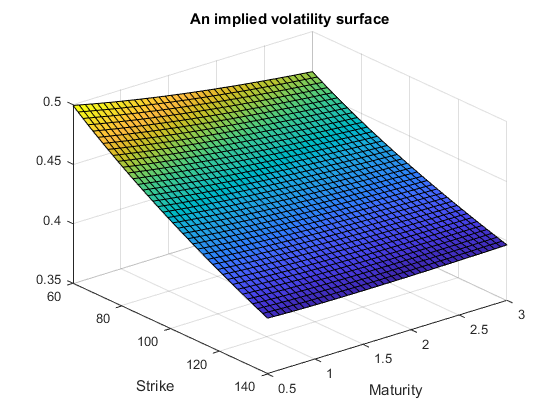
\includegraphics [width=4in]{fig/ScriptM_01.png}


\subsection{The local volatility surface}

\begin{par}
The goal of this section is to compute the local volatility by using the Dupire or BBF formula. We will use the output of the previous section.
\end{par} \vspace{1em}
\begin{par}
We can either compute the local volatility surface by using the prices and the Dupire formula or by using the implied volatility surface and the BBF formula. In this case we are using the Dupire formula. The function locVolSurf returns the local volatility surface, if we pass the input data (in our case the prices), the strike prices, the maturities, the risk free interest rate, the divident yield and a parameter which determines the used formula.
\end{par} \vspace{1em}
\begin{verbatim}
method = 'DUPIRE';
locVol = locVolSurf(K, T, r, q, PriceSurface, method, S0);
\end{verbatim}
\begin{par}
The following picture shows a surface plot of the computed local volatility surface.
\end{par} \vspace{1em}
\begin{verbatim}
surf(K(2:end-2),T(2:end-2),locVol)
view([50.9000 33.2000])
title('A local volatility surface')
ylabel('Maturity')
xlabel('Strike')
\end{verbatim}

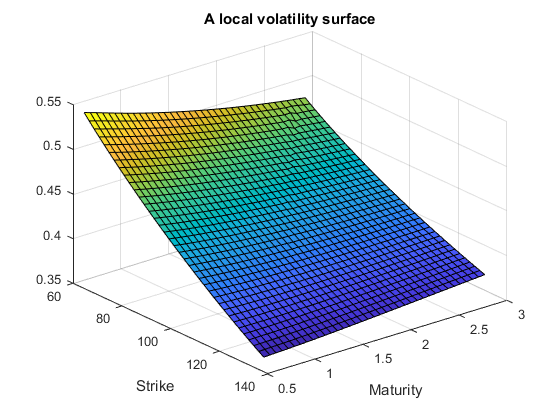
\includegraphics [width=4in]{fig/ScriptM_02.png}


\subsection{Practical use of the local volatility}

\begin{par}
Now we are going to use the local volatility in a Monte Carlo Euler simulator. In practice one can use the presented routine to price other, e.g. exotic derivatives. Our goal is to reprice the call options and to verify that the simulated call option prices match those we generated two sections ago (approximately). To simulate the price paths, we are going to use a modified version of the standard Euler scheme. We pass the local volatility surface, the other usual data and a parameter "Handle" to the function BSEulerMod. The Handle argument defines the action for the case when the simulated stock prices exceed the boundaries of the local volatility surface. If we pass TRUNC as Handle, the function will push the stocks prices back into the boundaries if the value of the simulated prices gets too big or too small. If we pass STOPS, the script will just ignore all the paths exceeding the boundaries.
\end{par} \vspace{1em}
\begin{verbatim}
Handle = 'NONE';
simN = 100000; % 100000 simulations
SimPrices = BSEulerMod(simN,dt,S0,K,T,r,q,locVol,Handle);
\end{verbatim}
\begin{par}
Now we compute the Call prices by using the CallPutPricer and compare the results to the original prices by calculating the relative error.
\end{par} \vspace{1em}
\begin{verbatim}
simPriceSurf = zeros(length(T)-3,length(K)-3);
for i = 3:length(T)-1
    for j = 2:length(K)-2
        simPriceSurf(i-2,j-1) = CallPutPricer(S0,...
        	SimPrices(:,i-1),K(j),T(i),r,q);
    end
end
RelError = abs(simPriceSurf-PriceSurface(3:length(T)-1,...
	2:length(K)-2))./PriceSurface(3:39,2:38);
\end{verbatim}
\begin{par}
The following picture shows the relative error of the simulated prices, computed without emergency stops and without truncation values.
\end{par} \vspace{1em}
\begin{verbatim}
surf(K(2:end-2),T(3:end-1),RelError)
title('Relative error')
ylabel('Maturity')
xlabel('Strike')
\end{verbatim}

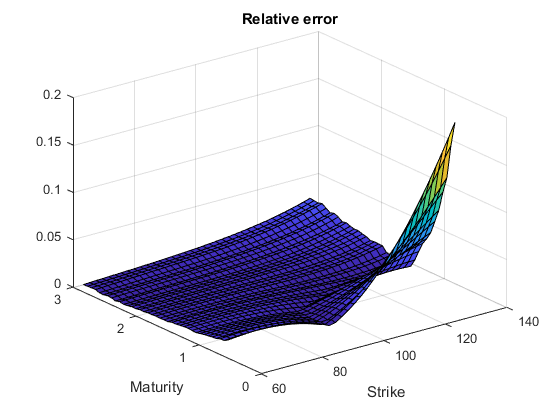
\includegraphics [width=4in]{fig/ScriptM_03.png}
\begin{par}
To see how emergency stops and truncation values effect the simulation, we plot the relative errors of all three methods into one figure.
\end{par} \vspace{1em}
\begin{verbatim}
surf(K(2:end-2),T(3:end-1),RelError)
title('Relative error comparison')
ylabel('Maturity')
xlabel('Strike')
hold

Handle = 'TRUNC';
SimPrices = BSEulerMod(simN,dt,S0,K,T,r,q,locVol,Handle);
simPriceSurf = zeros(length(T)-3,length(K)-3);
for i = 3:length(T)-1
    for j = 2:length(K)-2
        simPriceSurf(i-2,j-1) = CallPutPricer(S0,...
        	SimPrices(:,i-1),K(j),T(i),r,q);
    end
end
RelError = abs(simPriceSurf-PriceSurface(3:length(T)-1,...
	2:length(K)-2))./PriceSurface(3:39,2:38);
surf(K(2:end-2),T(3:end-1),RelError)

Handle = 'STOPS';
SimPrices = BSEulerMod(simN,dt,S0,K,T,r,q,locVol,Handle);
simPriceSurf = zeros(length(T)-3,length(K)-3);
for i = 3:length(T)-1
    for j = 2:length(K)-2
        simPriceSurf(i-2,j-1) = CallPutPricer(S0,...
        	SimPrices(:,i-1),K(j),T(i),r,q);
    end
end
RelError = abs(simPriceSurf-PriceSurface(3:length(T)-1,...
	2:length(K)-2))./PriceSurface(3:39,2:38);
surf(K(2:end-2),T(3:end-1),RelError)
hold off
legend('NONE','TRUNC','STOPS')
view([42.500 32.400])
\end{verbatim}
    
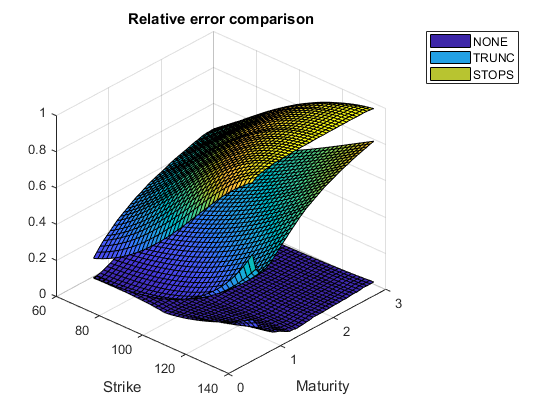
\includegraphics [width=4in]{fig/ScriptM_04.png}


\subsection{Implied volatility as "time-average" of the local volatility}

\begin{par}
As mentioned in a previous section, one can show that, under some technical conditions, the implied volatility is at large strikes approximately a time-average of the local volatility, i.g.
\end{par} \vspace{1em}
\begin{par}
$$I^2(t,x)=\frac{1}{t} \int_0^t (\sigma_u^\pm )^2du$$
\end{par} \vspace{1em}
\begin{par}
where $x(K,S) = \log\left(\frac{K}{S\exp\left(\mu t\right)}\right)$, $\sigma_t^\pm=\lim_{x\to\pm\infty}\sigma_t(x)$ and $I(t,x)$ denotes the implied volatility as a function of the log-forward-moneyness variable $x$.
\end{par} \vspace{1em}
\begin{par}
In this section we try to verify this formula. We do so by calculating the implied and local volatility for a high strikes and comparing both sides of the formula. We need to respecify the model parameter to meet the technical conditions and compute the new prices.
\end{par} \vspace{1em}
\begin{verbatim}
n=50;
T = (0.1:0.1:n*0.1)';
Kmin=60;
Kmax=150;
dk=(Kmax-Kmin)/(n-1);
K=(Kmin:dk:Kmax)';
paramsHeston = [0.05,0.5,0.2,0.001,-0.8];
[surface, PriceSurface] = ImplVolSurf(S0, K, T, r, q,...
	 paramsHeston, 'HESTON');
locSurf = locVolSurf(K,T,r,q,PriceSurface,'DUPIRE');
\end{verbatim}
\begin{par}
We approximate the integral by integrating numerically and we calculate a relative error like we did in the previous section.
\end{par} \vspace{1em}
\begin{verbatim}
integrand = locSurf(:,end).^2;
ImplVolAppr = ones(length(T)-4,1);
for i = 3:length(T)-2
    ImplVolAppr(i-2) = sqrt(1/T(i)*trapz(T(2:i),integrand(1:i-1)));
end
RelAppError = abs(ImplVolAppr-surface(3:length(T)-2,end-2))/...
	surface(3:length(T)-2,end-2);
\end{verbatim}
\begin{par}
The following image shows the relative error of the approximations with respect to the maturity.
\end{par} \vspace{1em}
\begin{verbatim}
plot(T(3:end-2),RelAppError)
title('Relative error')
xlabel('Maturity')
\end{verbatim}

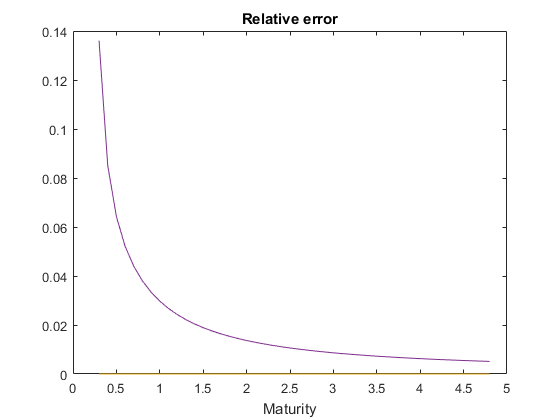
\includegraphics [width=4in]{fig/ScriptM_05.png}


\subsection{Implied volatility as "harmonic mean" of the local volatility}

\begin{par}
As allready mentioned, at very short maturity, the implied volatility at log-forward-moneyness $x$ is the harmonic mean of the local volatility across the moneyness dimension up to $x$, i.g.
\end{par} \vspace{1em}
\begin{par}
$$I^2(0,x) = \frac{x}{\int_0^x\frac{1}{\sigma_0^2(u)}du}.$$
\end{par} \vspace{1em}
\begin{par}
Now we proceed like we did in the previous section.
\end{par} \vspace{1em}
\begin{verbatim}
n=100; %no. of strike steps
T = (0.1:0.1:10*0.1)';
Kmin=100;
Kmax=130; %maximum value of strike price axis
dk=(Kmax-Kmin)/(n-1);
K=(Kmin:dk:Kmax)';

[surface, prices] = ImplVolSurf(S0, K, T, r, q,...
	 paramsHeston, 'HESTON');

locSurf = locVolSurf(K,T,r,q,prices,'DUPIRE');

integrand = 1./(locSurf(1,:).^2);
ImplVolAppr = zeros(length(K)-4,1);
for i = 3:length(K)-2
    ImplVolAppr(i-2) = sqrt(log(K(i)/S0)./(trapz(log(K(2:i)/S0),...
    	integrand(1:i-1))));
end
RelAppError = abs(ImplVolAppr-surface(2,3:length(K)-2))/...
	surface(2,3:length(K)-2);

plot(K(3:end-2),RelAppError)
title('Relative error')
xlabel('Strike')
\end{verbatim}

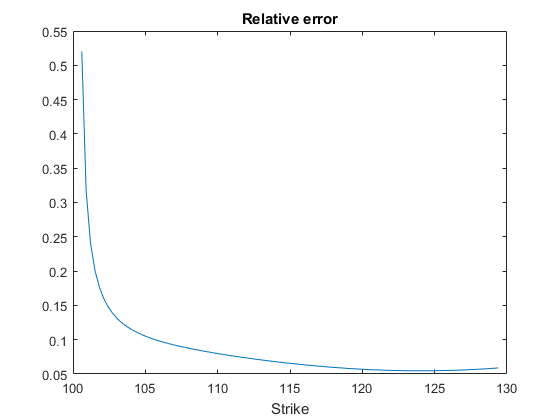
\includegraphics [width=4in]{fig/ScriptM_06.png}

\appendix

\section{Modified Code}
This section contains all MATLAB functions which we created or modified.

\subsection*{ImplVolSurf}
    \begin{verbatim}
function [surf, prices] = ImplVolSurf(S0, K, T, r, q, params, model)
%Creating the implied volatility surface for a prespecified model.

%S0: starting price
%K: strike of simulation
%T: time horizon of simulation
%r: riskfree rate
%q: dividend yield
%params: parameter of the model
%model: the used model, at the moment only 'HESTON' is available

%Author: Aaron Wittmann and Jan Keesen

% preallocating for speed
prices = zeros(length(T),length(K));
surf = zeros(length(T),length(K));

% Determine the model
switch(model)
    case 'HESTON'
        % The Transform is regular for im>1, so 1.1 is a reasonable choice
        im = 1.1;
        for i=1:length(T)
            for j=1:length(K)
                % calculating the price for different strikes K and
                % maturities T with Lewis Method
                prices(i,j) = CallPricingLewis(S0, K(j), T(i), r, q, params, im, model);
                surf(i,j) = BSimpVolFzero(S0, K(j), T(i), r, prices(i,j), q);
            end
        end
    otherwise
        error('This function does not support the passed variable.')
end
end
\end{verbatim}

\subsection*{CallPricingLewis}

    \begin{verbatim}
function call = CallPricingLewis(S0, K,T,r,q, params, im, model)
%Fourier inversion method using Lewis approach

%S0: spot price
%K: strike price
%T: time to matruity
%r: riskfree rate
%q: dividend yield

%params: model params (see the cf .m file)
%model: stochastic model used
%trunc: value of numerical integral truncation

%%Bonus: im>1 call price: im<0 putprice

%Author: Lorenzo Torricelli
%Modified by Aaron Wittmann and Jan Keesen

i=1i;
integrand = @(x)cfLibrary(-(x+i*im),S0,T,r,q,params, model).*K.^(1+i.*(x+i*im))./(i.*(x+i*im)-(x+i*im).^2);

% Relative error of 0.1%
call = .5*exp(-r*T)/pi * integral(integrand,-Inf,Inf,'AbsTol',1e-6,'RelTol',1e-4);
call=abs(call);
end
\end{verbatim}

\subsection*{BSimpVolFzero}
\begin{verbatim}
function [impliedVol] = BSimpVolFzero(S0,K,T,r, marketValue,q)
% Black-Scholes implied volatility.

%S0: spot price
%K: strike price
%r: riskFree rate
%T: time to maturity
%marketValue: observed call option market value
%q: stock dividend yield

%using fzero.

%Adapted by Lorenzo Torricelli
%Modified by Aaron Wittmann and Jan Keesen

impliedVol = ones(length(T),length(K));
for i = 1:length(T)
    it = BSimpVolAnalyticBrSu(S0, T(i),marketValue);
    for j = 1:length(K)
        fun = @(x) 	BSprice(S0, K(j), r, T(i), x, q)-marketValue;
        impliedVol(i,j) = fzero(fun,it);
    end
end

return
\end{verbatim}

\subsection*{locVolSurf}
\begin{verbatim}
function surf = locVolSurf(K, T, r, q, inputData, method, S0)
% This function computes the local volatility surface by using either
% Dupires formula or the BBF formula.

%If the Dupire-formula is used, the following parameters are used:
%K: strike price
%T: time horizon
%r: riskfree rate
%q: dividend yield
%inputData: price-matrix or implied volatility matrix

%If the BBF formula is used, the additional parameter is:
%S0: starting price

%method: the used method. Either BBF or DUPIRE.

%Author: Aaron Wittmann and Jan Keesen

switch method
    case 'DUPIRE'
        surf = localVolFromPrices(K,T, r , q, inputData);
    case 'BBF'
        if(~(nargin == 7))
            error('The amount of passed parameters is not correct.')
        end
        surf = localVolFromImplVol(S0, K, T, r, q, inputData);
    otherwise
        error('The passed method parameter is not valid. It has to be either DUPIRE or BBF.')
end
end
\end{verbatim}

\subsection*{BSEulerMod}
\begin{verbatim}
function price = BSEulerMod(simN, dt, S0,K, T, r, q, locSurf, Handle)
%Euler scheme for the Black Scholes model

%simN: number of simulations
%stepsN: number of time steps
%S0: starting price
%T: time horizon of simulation
%r: riskfree rate
%q: dividend yield
%sigma: volatility

%Author: Lorenzo Torricelli
%Modiefied by Aaron Wittmann and Jan Keesen

%rng(123, 'twister'); %seeding the Mersenne Twister


%Create first stock price
price=S0*ones(simN, length(T)-2);
drift=(r-q)*T(3)*ones(simN,1); %at time 0 there is no evolution
dWt=normrnd(0,1,simN, 1);
Kind = find(abs(S0-K(2:end-2))==min(abs(S0-K(2:end-2))),1,'first');
sigma = locSurf(1,Kind);
diffusion=sigma.*sqrt(T(3)).*dWt;
price(:, 2)=price(:, 1)+ price(:, 1).*(drift+diffusion);

if strcmp(Handle, 'TRUNC')==1
    price(price(:,2)>150,2) = 150;
    price(price(:,2)<50,2) = 50;
end

%Create other stock prices
drift=(r-q)*dt*ones(simN,1);
for i = 3:length(T)-2
    [I,~] = find((abs(price(:, i-1)-K(2:end-2)')-min(abs(price(:, i-1)-K(2:end-2)'),[],2))'==0,simN,'first');
    sigma = locSurf(i-1,I)';
    dWt=normrnd(0,1,simN, 1);
    diffusion=sigma.*sqrt(dt).*dWt;
    price(:, i)=price(:, i-1)+ price(:, i-1).*(drift+diffusion);
    if strcmp(Handle, 'TRUNC')==1
        price(price(:,i)>170,i) = 170;
        price(price(:,i)<40,i) = 40;
    end
end

if strcmp(Handle,'STOPS')==1
    [I,~] = find(price>150|price<50);
    REM = unique(I);
    IND = setdiff(1:simN,unique(REM));
else
    IND = 1:simN;
end
price = price(IND,:);

return
\end{verbatim}
\section{Used Code}
This section contains a list of all MATLAB functions we did use but not create or modify.
\begin{itemize}
\item BSimpVolAnalyticBrSu 
\item BSprice
\item CallPutPricer
\item cfLibrary
\item localVolFromImplVol
\item localVolFromPrices
\end{itemize}

%%%%%%%%%%%%%%%%%%%%%%%%%%%%%%%%%%%%%%%%%%%%%%
%%    End of the main document              %%
%%%%%%%%%%%%%%%%%%%%%%%%%%%%%%%%%%%%%%%%%%%%%%
\newpage
%\bibliographystyle{abbrvdin}
%\bibliography{refs}

\end{document}